\documentclass[journal,12pt,twocolumn]{IEEEtran}
%
\usepackage{setspace}
\usepackage{gensymb}
%\doublespacing
\singlespacing

%\usepackage{graphicx}
%\usepackage{amssymb}
%\usepackage{relsize}
\usepackage[cmex10]{amsmath}
\usepackage{siunitx}
%\usepackage{amsthm}
%\interdisplaylinepenalty=2500
%\savesymbol{iint}
%\usepackage{txfonts}
%\restoresymbol{TXF}{iint}
%\usepackage{wasysym}
\usepackage{amsthm}
\usepackage{iithtlc}
\usepackage{mathrsfs}
\usepackage{txfonts}
\usepackage{stfloats}
\usepackage{steinmetz}
%\usepackage{bm}
\usepackage{cite}
\usepackage{cases}
\usepackage{subfig}
%\usepackage{xtab}
\usepackage{longtable}
\usepackage{multirow}
%\usepackage{algorithm}
%\usepackage{algpseudocode}
\usepackage{enumitem}
\usepackage{mathtools}
\usepackage{tikz}
\usepackage{circuitikz}
\usepackage{pgfplots}
\usepackage{verbatim}
\usepackage{tfrupee}
\usepackage[breaklinks=true]{hyperref}
%\usepackage{stmaryrd}
\usepackage{tkz-euclide} % loads  TikZ and tkz-base
%\usetkzobj{all}
\usetikzlibrary{calc,math}
\usetikzlibrary{fadings}
\usepackage{listings}
    \usepackage{color}                                            %%
    \usepackage{array}                                            %%
    \usepackage{longtable}                                        %%
    \usepackage{calc}                                             %%
    \usepackage{multirow}                                         %%
    \usepackage{hhline}                                           %%
    \usepackage{ifthen}                                           %%
  %optionally (for landscape tables embedded in another document): %%
    \usepackage{lscape}     
\usepackage{multicol}
\usepackage{chngcntr}
%\usepackage{enumerate}

%\usepackage{wasysym}
%\newcounter{MYtempeqncnt}
\DeclareMathOperator*{\Res}{Res}
%\renewcommand{\baselinestretch}{2}
\renewcommand\thesection{\arabic{section}}
\renewcommand\thesubsection{\thesection.\arabic{subsection}}
\renewcommand\thesubsubsection{\thesubsection.\arabic{subsubsection}}

\renewcommand\thesectiondis{\arabic{section}}
\renewcommand\thesubsectiondis{\thesectiondis.\arabic{subsection}}
\renewcommand\thesubsubsectiondis{\thesubsectiondis.\arabic{subsubsection}}

% correct bad hyphenation here
\hyphenation{op-tical net-works semi-conduc-tor}
\def\inputGnumericTable{}                                 %%

\lstset{
%language=C,
frame=single, 
breaklines=true,
columns=fullflexible
}
%\lstset{
%language=tex,
%frame=single, 
%breaklines=true
%}

\begin{document}
%


\newtheorem{theorem}{Theorem}[section]
\newtheorem{problem}{Problem}
\newtheorem{proposition}{Proposition}[section]
\newtheorem{lemma}{Lemma}[section]
\newtheorem{corollary}[theorem]{Corollary}
\newtheorem{example}{Example}[section]
\newtheorem{definition}[problem]{Definition}
%\newtheorem{thm}{Theorem}[section] 
%\newtheorem{defn}[thm]{Definition}
%\newtheorem{algorithm}{Algorithm}[section]
%\newtheorem{cor}{Corollary}
\newcommand{\BEQA}{\begin{eqnarray}}
\newcommand{\EEQA}{\end{eqnarray}}
\newcommand{\define}{\stackrel{\triangle}{=}}

\bibliographystyle{IEEEtran}
%\bibliographystyle{ieeetr}


\providecommand{\mbf}{\mathbf}
\providecommand{\pr}[1]{\ensuremath{\Pr\left(#1\right)}}
\providecommand{\qfunc}[1]{\ensuremath{Q\left(#1\right)}}
\providecommand{\sbrak}[1]{\ensuremath{{}\left[#1\right]}}
\providecommand{\lsbrak}[1]{\ensuremath{{}\left[#1\right.}}
\providecommand{\rsbrak}[1]{\ensuremath{{}\left.#1\right]}}
\providecommand{\brak}[1]{\ensuremath{\left(#1\right)}}
\providecommand{\lbrak}[1]{\ensuremath{\left(#1\right.}}
\providecommand{\rbrak}[1]{\ensuremath{\left.#1\right)}}
\providecommand{\cbrak}[1]{\ensuremath{\left\{#1\right\}}}
\providecommand{\lcbrak}[1]{\ensuremath{\left\{#1\right.}}
\providecommand{\rcbrak}[1]{\ensuremath{\left.#1\right\}}}
\theoremstyle{remark}
\newtheorem{rem}{Remark}
\newcommand{\sgn}{\mathop{\mathrm{sgn}}}
\providecommand{\abs}[1]{\left\vert#1\right\vert}
\providecommand{\res}[1]{\Res\displaylimits_{#1}} 
\providecommand{\norm}[1]{\left\lVert#1\right\rVert}
%\providecommand{\norm}[1]{\lVert#1\rVert}
\providecommand{\mtx}[1]{\mathbf{#1}}
\providecommand{\mean}[1]{E\left[ #1 \right]}
\providecommand{\fourier}{\overset{\mathcal{F}}{ \rightleftharpoons}}
%\providecommand{\hilbert}{\overset{\mathcal{H}}{ \rightleftharpoons}}
\providecommand{\ztrans}{\overset{\mathcal{Z}}{ \rightleftharpoons}}
\providecommand{\system}{\overset{\mathcal{H}}{ \longleftrightarrow}}
	%\newcommand{\solution}[2]{\textbf{Solution:}{#1}}
\newcommand{\solution}{\noindent \textbf{Solution: }}
\newcommand{\cosec}{\,\text{cosec}\,}
\providecommand{\dec}[2]{\ensuremath{\overset{#1}{\underset{#2}{\gtrless}}}}
\newcommand{\myvec}[1]{\ensuremath{\begin{pmatrix}#1\end{pmatrix}}}
\newcommand{\mydet}[1]{\ensuremath{\begin{vmatrix}#1\end{vmatrix}}}
\providecommand{\gauss}[2]{\mathcal{N}\ensuremath{\left(#1,#2\right)}}
%\providecommand{\system}[1]{\overset{\mathcal{#1}}{ \longleftrightarrow}}
\newcommand*{\permcomb}[4][0mu]{{{}^{#3}\mkern#1#2_{#4}}}
\newcommand*{\perm}[1][-3mu]{\permcomb[#1]{P}}
\newcommand*{\comb}[1][-1mu]{\permcomb[#1]{C}}

\title{
%\logo{
GATE Problems in Probability
%}
}

\maketitle

\begin{abstract}
These problems have been selected from GATE question papers and can be used for conducting tutorials in courses related to a first course in probability.
\end{abstract}
%\centering \textbf{\Large Probability}\\

\begin{enumerate}
\setlength\itemsep{2em}

\item Let X be a random variable with the following cumulative distribution function:
\begin{align}
F\brak{x} 
= 
\begin{cases}
0           & x < 0 \\
x^2         & 0 \leq x < \frac{1}{2} \\
\frac{3}{4} & \frac{1}{2} \leq x < 1 \\
1           &  x \geq 1 
\end{cases}
\end{align}
Then $ P\brak{\frac{1}{4} < X < 1}$ is equal to

%
\solution

\begin{align}
    P\brak{\frac{1}{4} < X < 1} &= F\brak{1^{-}}-F\brak{\frac{1}{4}} \\
    &= \frac{3}{4} - \brak{\frac{1}{4}}^{2}\\
    &= \frac{11}{16}
\end{align}
\begin{figure}[!ht]
\centering
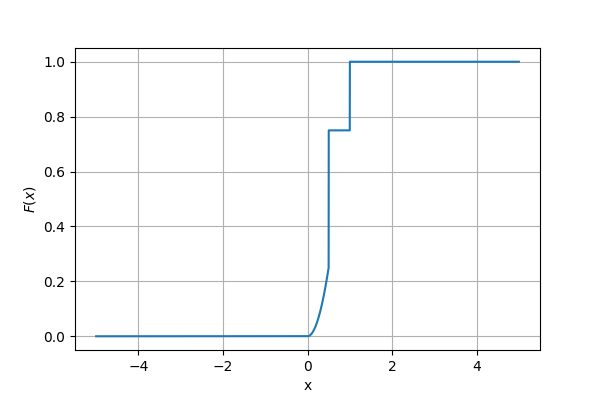
\includegraphics[width=\columnwidth]{solutions/ma/2016/30/figs/Assignment4_CDF.png}
\caption{The CDF of X}
\label{cdf}
\end{figure}



\item Let X and Y be continuous random variables with the joint probability density function 
\begin{align}
f\brak{x,y}= 
\begin{cases}
ae^{-2y} & 0<x<y<\infty \\
0 & \text{otherwise}.
\end{cases}   
\end{align}
Then $E\brak{X|Y=2}$ is \dots
\solution
Given X and Y are two continuous random variables with joint probability density function,
\begin{align}
f\brak{x,y}= 
\begin{cases}
ae^{-2y} & 0<x<y<\infty \\
0 & \text{otherwise}.
\end{cases}   
\end{align}
% \begin{figure}[!hbt]
%     \centering
%     \includegraphics[width=\columnwidth]{Figure_0.png}
%     \caption{Graph of x=y}
%     \label{Figure_1}
% \end{figure}
We know that,\\
$0<x<y<\infty  \implies x<y<\infty \text{ for } 0<x<\infty.$\\ 
Then,
\begin{align}
    f_X\brak{x} &= \int f_{XY}\brak{x,y}dy\\
    &= \int_{x}^{\infty} ae^{-2y}dy\\
    &= \left[ \frac{ae^{-2y}}{(-2)} \right]_{x}^{\infty}\\
    &= \frac{-a}{2}\left[ e^{-2y}\right]_{x}^{\infty}\\
    &= \frac{-a}{2}[0-e^{-2x}]\\
\implies f_X\brak{x} &=
    \begin{cases}
    \frac{a}{2}e^{-2x} & 0 < x < \infty\\
    0 & \text{otherwise}.
    \end{cases}
\end{align}
Similarly,\\
$ 0<x<y<\infty \implies 0<x<y \text{ for } 0<y<\infty$ \\
Then,
\begin{align}
    f_y\brak{y} &= \int f_{XY}\brak{x,y}dx\\
    &= \int_{0}^{y} ae^{-2y}dx\\
    &= ae^{-2y}[x]_{0}^{y}\\
    &= aye^{-2y}\\
\implies f_Y\brak{y} &=
    \begin{cases}
    aye^{-2y} & 0 < y < \infty\\
    0 & \text{otherwise}.
    \end{cases}
\end{align}
%\begin{figure}[ht]
%    \centering
%    \includegraphics[width=\columnwidth]{Figure_1.png}
%    \caption{Graph of x+y=1}
%    \label{Figure_1}
%\end{figure}
Therefore ,
\begin{align}
    f_{X|Y}\brak{x|y} &= \frac{f_{XY}\brak{x,y}}{f_Y\brak{y}}\\
    & = \frac{ae^{-2y}}{aye^{-2y}}\\
    & = \frac{1}{y}\\
\implies f_{X|Y}\brak{x|y} &=
    \begin{cases}
    \frac{1}{y} & \text{if } 0<x<y<\infty\\
    0 & \text{otherwise}
    \end{cases}
\end{align}
Then, 
\begin{align}
   E\brak{X|Y=y} & =
   \int_{-\infty}^{\infty} (x)f_{X|Y}\brak{x|y}dx\\
    & = \int_{0}^{y}(x)\brak{\frac{1}{y}}dx\\
    & = \frac{1}{y} \int_{0}^{y}(x)dx \\
    & = \frac{1}{y} \left[ \frac{x^2}{2}\right]_{0}^{y}\\
    & = \frac{1}{y}\brak{\frac{y^2}{2}}\\
    & = \frac{y}{2}\\
\implies E\brak{X|Y=y} &= \frac{y}{2}\\
\therefore E\brak{X|Y=2} &= 1
\end{align}
%
\item A continuous random variable X has the probability density function
\begin{align*}
    f(x) &= \begin{cases} 
      \frac{3}{5}e^{-\frac{3}{5}x} & x > 0 \\
      0 & x\leq 0\\
   \end{cases} 
\end{align*} 
The probability density function of $Y=3X+2$  is
\begin{enumerate}
    \item \begin{align*}
         f(y) &= \begin{cases} 
      \frac{1}{5}e^{-\frac{1}{5} (y-2)} & y > 2 \\
      0 & y \leq 2\\
   \end{cases} 
    \end{align*}
\item \begin{align*}
    f(y) &= \begin{cases} 
      \frac{2}{5}e^{-\frac{2}{5} (y-2)} & y > 2 \\
      0 & y \leq 2\\
   \end{cases} 
\end{align*} 
\item  \begin{align*}
    f(y) &= \begin{cases} 
      \frac{3}{5}e^{-\frac{3}{5} (y-2)} & y > 2 \\
      0 & y \leq 2\\
   \end{cases} 
\end{align*} 
\item \begin{align*}
    f(y) &= \begin{cases} 
      \frac{4}{5}e^{-\frac{4}{5} (y-2)} & y > 2 \\
      0 & y \leq 2\\
   \end{cases} 
\end{align*} 
\end{enumerate}
%
\solution
Given $Y=3X+2$ \\
    CDF of $Y$, 
    \begin{align*}
        F_y(Y) &= \Pr(Y\leq y) \\
        &= \Pr\left(X \leq \frac{y-2}{3} \right) \\
        &= F_x\left(\frac{y-2}{3}\right) \\
    \end{align*}
    Thus, pdf of $Y$ ,\begin{align*}
        f_Y(y) &= \frac{1}{3}f_X\left(\frac{y-2}{3}\right)\\
        &= \frac{1}{3} \times \begin{cases} \frac{3}{5}e^{-\frac{3}{5}\left(\frac{y-2}{3}\right)}  & y>2 \\
        0 & y \leq 2 \\\end{cases}\\
        &= \begin{cases} 
      \frac{1}{5}e^{-\frac{1}{5} (y-2)} & y > 2 \\
      0 & y \leq 2\\
   \end{cases} 
    \end{align*}
Hence, correct option is 1. 
%
\item    Let the probability density function of a random variable X be
   $$
   f(x)=
   \begin{cases}
   x~~~~~~~~~~~~~~~0\leqslant x < \dfrac{1}{2}\\
   c(2x-1)^2~~~~~\dfrac{1}{2}\leqslant x <1\\
   0 ~~~~~~~~~~~~~~~\text{Otherwise}
   \end{cases}
   $$
   Then value of c is equal to ...
   \\
\solution
We know that,
\begin{align}
\int_{-\infty}^{\infty}{f_x(x)}\,dx &= 1\\
    \int_{-\infty}^{0}{f_x(x)}\,dx +\int_{0}^{\frac{1}{2}}{f_x(x)}\,dx&\nonumber\\ +\int_{\frac{1}{2}}^{1}{f_x(x)}\,dx +\int_{1}^{\infty}{f_x(x)}\,dx&=1\\
    \int_{0}^{\frac{1}{2}}x\,dx+\int_{\frac{1}{2}}^{1}c(2x-1)^2\,dx&=1\\
    \sbrak{\dfrac{x^2}{2}}_0^\frac{1}{2}+c \sbrak{\dfrac{(2x-1)^3}{6}}_\frac{1}{2}^1&=1\\
    \dfrac{1}{8}+\dfrac{c}{6}&=1\\
    c&=\dfrac{21}{4}
\end{align}
\hspace{2cm}$\therefore$ Required value of $c=\dfrac{21}{4}$

\begin{figure}[h]
   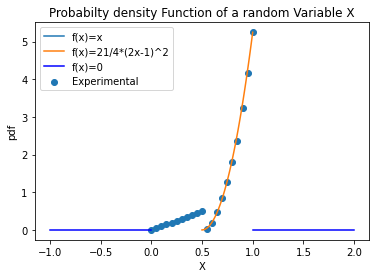
\includegraphics[width=\linewidth]{solutions/ma/2016/10/figures/plot.png}
    \caption{Experimental and Theoritical pdf of X}
    \label{fig:my_label}
\end{figure}




%
\item Let $A_{1},A_{2},.....A_{n}$ be n independent events in which the Probability of occurence of the event $A_{i}$ is given by P($A_{i}$) = 1 - $\frac{1}{\alpha^i}$, $\alpha >1$, i = 1,2,3,....n.Then the probability that atleast one of the events occurs is
\begin{enumerate}
    \item  1 - $\frac{1}{\alpha^\frac{n(n+1)}{2}}$ \hspace{0.95cm}
    \item  $\frac{1}{\alpha^\frac{n(n+1)}{2}}$\hspace{1.5cm}
    \\ \\
    \item  $\frac{1}{\alpha^n}$ \hspace{2.15cm}
    \item 1 - $\frac{1}{\alpha^n}$\hspace{0.95cm}
  \end{enumerate}
  %
  \solution
  Let $A_{1} + A_{2} + A_{3} .... + A_{n}$ = S, \\
$\pr{S}$ = Probability of atleast one event occuring
De morgan's law states that $(A + B)^\prime = A^\prime B^\prime$  
\begin{align}
    \label{1.1}
   \implies \pr{S} = 1 - \pr{S^\prime} \\ 
   %\label{1.2}
   1 - \pr{S^\prime}= 1 - \pr{A_{1}^\prime A_{2}^\prime A_{3}^\prime
   ....A_{n}^\prime}
   \label{ma2005:1}
\end{align}
$\forall$ i $\in$ {1,2,....n} \\
Since, $A_{i}$ are independent.\\
$\therefore$ Complements of $A_{i}$ are also independent.\\
$\implies$ 
\begin{equation}
%\label{2.1}
\pr{A_{1}^\prime A_{2}^\prime A_{3}^\prime
   ....A_{n}^\prime}=\prod_{i=1}^{n}\pr{A_{i}^\prime}
   \label{ma2005:2}
\end{equation}
\begin{equation}
%    \label{2.2}
\pr{A_{i}} = 1 - \frac{1}{\alpha^i} \implies \pr{A_{i}^\prime} = \frac{1}{\alpha^i} \label{ma2005:5}
\end{equation}
substituting \eqref{ma2005:5} in \eqref{ma2005:2},
\begin{equation}
    \label{2.3}
  \pr{A_{1}^\prime A_{2}^\prime A_{3}^\prime ....A_{n}^\prime} =  \prod_{i=1}^{n}\frac{1}{\alpha^i} \\
\end{equation}
\begin{equation}
\label{2.4}
   \prod_{i=1}^{n}\frac{1}{\alpha^i}=\frac{1}{\alpha^{\sum_{i}^{n}i}}= \frac{1}{\alpha^\frac{n(n+1)}{2}} 
\end{equation}
\begin{equation}
%\label{2.5}
    \therefore \pr{A_{1}^\prime A_{2}^\prime A_{3}^\prime ....A_{n}^\prime} = \pr{S^\prime} = \frac{1}{\alpha^\frac{n(n+1)}{2}} \label{ma2005:3}
\end{equation}
from equations \eqref{ma2005:1} and \eqref{ma2005:3} 
\begin{equation}
\label{2.6}
\implies \pr{S} = 1 - \pr{S^\prime} = 1 - \frac{1}{\alpha^\frac{n(n+1)}{2}}
\end{equation}
$\therefore$ The correct option is \textbf{(a)}
  %
  \item Let the random variable X have the distribution function 
$F(x)= \begin{cases}
       0  & if \:x<0\\
       \frac{x}{2} & if\: 0 \le x <1\\
       \frac{3}{5} & if \:1 \le x <2\\
       \frac{1}{2} +\frac{x}{8} & if\: 2\le x <3\\
       1  & if\: x\ge 3
    \end{cases}$\\
Then $\pr{2\le x <4}$ is equal to 
%
\\
  \solution
  
Given,
\begin{align}
F(x)= \begin{cases} 
       0  & if \:x<0\\
       \frac{x}{2} & if\: 0 \le x <1\\
       \frac{3}{5} & if \:1 \le x <2\\
       \frac{1}{2} +\frac{x}{8} & if\: 2\le x <3\\
       1  & if\: x\ge 3
    \end{cases} \label{a}
\end{align}
We need to find $\pr{2\le x <4}$,which is also can be written as
\begin{align}
\pr{2\le x <4} &= \pr{x<4} - \pr{ x <2}\\
              &= F(X=4^{-}) - F(X=2^{-})\label{b}
 \end{align} 
 Using \eqref{a} in \eqref{b},
 \begin{align}
 \pr{2\le x <4} &= 1 - \frac{3}{5}\\
                &= \frac{2}{5}\\
                &= 0.4 
\end{align} 


\begin{figure}[ht]
    \centering
    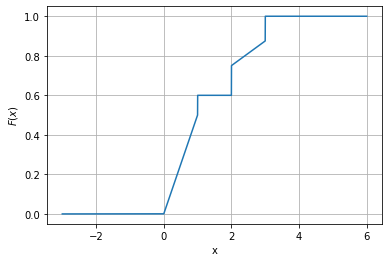
\includegraphics[width=\columnwidth]{solutions/ma/2015/9/Fig_assign_5.png}
    \caption{cdf of random variable X}
\end{figure}

\item Let Z be the vertical coordinate, between -1 and 1, of a point chosen uniformly at random on the
\begin{math}
\text{surface of a unit sphere in }R^3.\text{ Then,} \pr{\frac{-1}{2} \leq Z \leq \frac{1}{2}}
\end{math}
is
\\
  \solution
  The equation of the sphere can be written as :
\begin{math}
x^2 + y^2 + z^2 = 1.
\end{math}
Now,
\begin{align}
\pr{\frac{-1}{2} \leq z \leq 0}&=\pr{0 \leq z^2 \leq \frac{1}{4}}
\\\pr{0 \leq z \leq \frac{1}{2}}&=\pr{0 \leq z^2 \leq \frac{1}{4}}
\\\therefore \pr{\frac{-1}{2} \leq z \leq \frac{1}{2}}&=2 \times \pr{0 \leq z^2 \leq \frac{1}{4}}
\end{align}
\begin{align}
\pr{0 \leq z^2 \leq \frac{1}{4}}&=\pr{\frac{3}{4} \leq x^2+y^2 \leq 1}
\\\text{Taking, } x^2+y^2&=r^2.
\end{align}
\begin{align}
     \pr{\frac{3}{4} \leq r^2 \leq 1} &= \frac{1}{4}
\end{align}
     \brak{ \text{Since, }r^2 \text{ is uniform between 0 and 1} }
\begin{align}
     \therefore \pr{\frac{-1}{2} \leq Z \leq \frac{1}{2}} &= 2 \times \frac{1}{4} = \frac{1}{2}
\end{align}
%
\item Let $X_1$ and $X_2$ be independent geometric random variables with the same probability
mass function given by $\pr{X = k} = p(1-p)^{k-1}$
, $k = 1, 2, \ldots$ Then the value of
$\pr{X_1 = 2 | X_1 + X_2 = 4}$ correct up to three decimal places is
\\
  \solution
  Let 
\begin{align}
\label{eq:dice_pmf_xi}
p_{X_i}(k)=\pr{X_i=k}=
\begin{cases}
p(1-p)^{k-1} & n=1,2,...
\\
0 & otherwise
\end{cases}
\end{align}
where i=1,2
\begin{align}
\pr{A|B}=\frac{\pr{AB}}{\pr{B}}
\end{align}
\begin{align}
(X_1 = 2) \cap (X_1 + X_2 = 4)=\brak{X_1=2,X_2=2}
\end{align}
Thus,
\begin{align}
  \pr{X_1 = 2 | X_1 + X_2 = 4}&=\frac{\pr{X_1=2,X_2=2}}{\pr{X_1+X_2=4}}
 \end{align}
 Since the two events are independent,
\begin{align}\label{result}
  \pr{X_1 = 2 | X_1 + X_2 = 4}=\frac{\pr{X_1=2}\pr{X_2=2}}{\pr{X_1+X_2=4}}
 \end{align}
Let
\begin{align}\label{eq:dice_xdef}
X=X_1+X_2
\end{align}
From \eqref{eq:dice_xdef},
\begin{align}
p_X(n) &= \pr{X_1 + X_2 = n} = \pr{X_1  = n -X_2}
\\
&= \sum_{k}^{}\pr{X_1  = n -k | X_2 = k}p_{X_2}(k)
\label{eq:dice_x_sum}
\end{align}
after unconditioning.  $\because X_1$ and $X_2$ are independent,
\begin{multline}
\pr{X_1  = n -k | X_2 = k} 
\\
= \pr{X_1  = n -k}
= p_{X_1}(n-k)
\label{eq:dice_x1_indep}
\end{multline}
From \eqref{eq:dice_x_sum} and \eqref{eq:dice_x1_indep},
\begin{align}
p_X(n) = \sum_{k}^{}p_{X_1}(n-k)p_{X_2}(k) = p_{X_1}(n)*p_{X_2}(n)
\label{eq:dice_x_conv}
\end{align}
where $*$ denotes the convolution operation. 
%\cite{proakis_dsp}.  
Substituting from \eqref{eq:dice_pmf_xi}
in \eqref{eq:dice_x_conv},
\begin{align}
p_X(n)& = \sum_{k=1}^{n-1}p_{X_1}(n-k)p_{X_2}(k)\\
& = \sum_{k=1}^{n-1} (1-p)^{k-1} p \cdot (1-p)^{n-k-1} p \\ & = (1-p)^{n-2} p^2 \sum_{k=1}^{n-1} 1 \\& = (n-1) (1-p)^{n-2}p^2\label{ref}\end{align}
From \eqref{ref} and \eqref{eq:dice_pmf_xi} we have
\begin{align}
&\pr{X_1=2}=\pr{X_2=2}=p(1-p)\\
&\pr{X_1+X_2=4}=3(1-p)^2p^2
\end{align}
Substituting in \eqref{result}
\begin{align}
 \pr{X_1 = 2 | X_1 + X_2 = 4}
 &=\frac{(1-p)^2p^2}{3(1-p)^2p^2}\\
 &=\frac{1}{3}
\end{align}
%
\item     Let X and Y have joint probability function given by\\
    $$f_{X,Y}(x,y)=\left\{
    \begin{array}{ll}
      2 & 0\leq x\leq 1-y,0\leq y\leq 1 \\
      0 & otherwise \\
    \end{array} 
    \right. $$
    If $f_{Y}$ denotes the marginal probability density function of Y, then $f_{Y}(1/2)=?$
\\
\solution

\begin{align}
    \tag{23.1}
    f_{Y}(y) = \int_{-\infty}^{\infty}f_{X,Y}(x,y).dx
\end{align}
\begin{align}
    \tag{23.2}
    \implies f_{Y}(y) = \left\{
    \begin{array}{ll}
      0+\int_{0}^{1-y}2.dx & 0\leq y\leq 1 \\
      0 & otherwise \\
    \end{array} 
    \right.
\end{align}
\begin{align}
    \tag{23.3}
    \implies f_{Y}(y) = \left\{
    \begin{array}{ll}
      2(1-y) & 0\leq y\leq 1 \\
      0 & otherwise \\
    \end{array} 
    \right.
\end{align}
\begin{align}
    \tag{23.4}
    \therefore f_{Y}(1/2) = 1
\end{align}
\begin{figure}
\centering
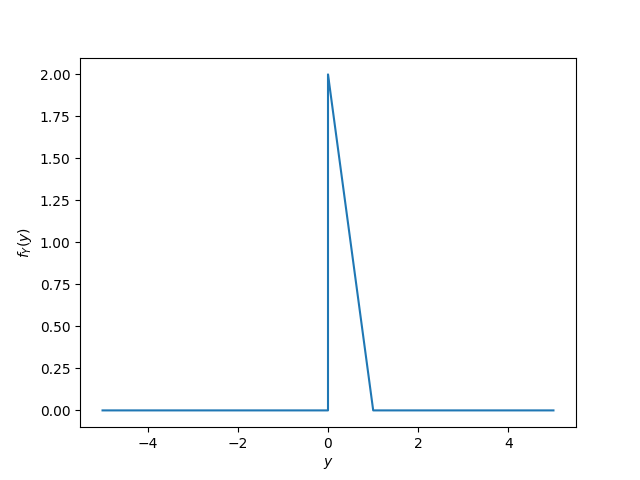
\includegraphics[width=\columnwidth]{solutions/ma/2018/23/Figure/Plot.png}
\caption{Marginal PDF}
\label{fig:ma2018-23:marginal}
\end{figure}



%
\item Let X be a standard normal random variable. Then $\pr{X < 0 |\;\abs{\lfloor X\rfloor} = 1}$ is equal to
\begin{enumerate}[label = \alph*)]
    \item $\cfrac{\Phi(1) - \frac{1}{2}}{\Phi(2) - \frac{1}{2}}$
    \item $\cfrac{\Phi(1) + \frac{1}{2}}{\Phi(2) + \frac{1}{2}}$
    \item $\cfrac{\Phi(1) - \frac{1}{2}}{\Phi(2) + \frac{1}{2}}$
    \item $\cfrac{\Phi(1) + 1}{\Phi(2) + 1}$
\end{enumerate}
%
\solution

\begin{align}
    &\abs{\lfloor X\rfloor} = 1\\
    \implies &\lfloor X\rfloor = 1\; or\; -1\\
    \implies &X \in [1, 2) \cup [-1, 0)
\end{align}
Here 
\begin{align*}
    \lfloor X\rfloor = greatest\; integer\; less\; than\; or\; equal\; to\; X
\end{align*}
Thus required probability
\begin{align}
    &= \frac{\pr{X\in [-1,0)}}{\pr{X \in [1, 2) \cup [-1, 0)}}
\end{align} 
Using symmetry of standard normal random variable about y = 0, we have required probability 
\begin{align}
    &= \cfrac{\pr{X\in (0,1]}}{\pr{X \in [1, 2) \cup (0, 1])}}\\
    &= \cfrac{\pr{X \in (0, 1]}}{\pr{X \in (0, 2)}}\\
    &= \cfrac{\pr{X < 1} - \pr{X < 0}}{\pr{X < 2} - \pr{X < 0}}\\
    &= \cfrac{\Phi(1) - \Phi(0)}{\Phi(2) - \Phi(0)}\\
    &= \cfrac{\Phi(1) - \frac{1}{2}}{\Phi(2) - \frac{1}{2}}\label{bato}\\
    &= \cfrac{0.841 - 0.5}{0.977 - 0.5}\label{gato}\\
    &= 0.715
\end{align}
Here $\Phi(x)$ represents the standard normal cumulative density function. Thus 
\begin{align}
    X \sim \mathcal{0}{1}
\end{align}
and 
\begin{align}
    \Phi(x) = \int_{-\infty}^x f_X(x)dx
\end{align}
It can easily be seen that $\Phi(0) = \frac{1}{2}$, which has been used to obtain \eqref{bato}.
\eqref{gato} was obtained by consulting tables for $\Phi(x)$
%
\item Let $X$ be a random variable with probability mass function 
$p(n) = \brak{\frac{1}{4}}\brak{\frac{3}{4}}^{n-1}  n=1,2 \ldots $ \\
Then $E[X-3|X>3]$ is \dots
\\
\solution

Given\begin{align}\label{ma2017-46:5}
\pr{X=n} = \begin{cases}
    \brak{\frac{1}{4}}\brak{\frac{3}{4}}^{n-1} & n=1,2 \ldots \\
    0 & otherwise
\end{cases}
\end{align}
Using the linearity of the expectation operator:
\begin{align}\label{ma2017-46:eq-1}
 E[X - 3 \mid X > 3] = E[X \mid X > 3] - 3
\end{align}
Now ,
\begin{align}
E[X \mid X > 3] &= \sum_{x=1}^{\infty} x  \pr{X=x \mid X > 3}\\
& = \sum_{x=1}^{\infty} x \frac{\pr{X=x, X > 3}}{\pr{X > 3}}\label{ma2017-46:eq1}
\end{align}
Calculating $\pr{X>3}$
\begin{align}
\pr{X > 3} =& 1 - \pr{X \leq 3}   \\
=& 1 - \sum_{x'=1}^3 \pr{X=x'} \\
=& 1 - \sum_{x'=1}^3 \brak{\frac{3}{4}}^{x'-1}\brak{\frac{1}{4}}\\
=& \frac{27}{64} \label{ma2017-46:eq2}
\end{align}
%Computing $P(X=x, X > 3)$
Also,\begin{align}\label{ma2017-46:eq3}
\pr{X=x, X > 3} = \begin{cases}
    \pr{X=x} & x > 3 \\
    0 & x \leq 3
\end{cases}
\end{align}
 %Combining the numerator and denominator
Substituting \eqref{ma2017-46:eq2} and \eqref{ma2017-46:eq3} in  \eqref{ma2017-46:eq1} we get
\begin{align}
E[X \mid X > 3] 
&= \sum_{x=1}^{3} 0 + \sum_{x=4}^{\infty} \sbrak{ x   \frac{\pr{X=x}}{\frac{27}{64}} } \\
&=\frac{64}{27} \sum_{x=4}^{\infty} \sbrak{  
x\brak{\frac{1}{4}}\brak{\frac{3}{4}}^{x-1}}\\
&=\frac{16}{27}\sum_{x=4}^{\infty} \sbrak{ x \brak{\frac{3}{4}}^{x-1}}\label{ma2017-46:sub}
\end{align}

Let
\begin{align}\label{ma2017-46:S}
S&=\sum_{x=4}^{\infty} \sbrak{ x \brak{\frac{3}{4}}^{x-1}}\
\end{align}
Multiplying (\eqref{ma2017-46:S}) with  $\frac{3}{4}$ on both sides gives
\begin{align}\label{ma2017-46:3/4S}
\frac{3}{4}S&=\sum_{x=4}^{\infty} x\frac{1}{4}\left(\frac{3}{4}\right)^{x} 
\end{align}
From \eqref{ma2017-46:3/4S} and\eqref{ma2017-46:S} 
\begin{align}
S&= 4 \brak{\frac{3}{4}}^{3}+5 \brak{\frac{3}{4}}^{4}+6 \brak{\frac{3}{4}}^{5}\ldots\\
\frac{3}{4}S&= 0\brak{\frac{3}{4}}^{3}+ 4 \brak{\frac{3}{4}}^{4}+5 \brak{\frac{3}{4}}^{5}+\ldots
\end{align}
subtracting \eqref{ma2017-46:3/4S} from \eqref{ma2017-46:S} we get
\begin{align}
\frac{S}{4}&= 4 \brak{\frac{3}{4}}^{3}+ \brak{\frac{3}{4}}^{4}+\brak{\frac{3}{4}}^{5}+\brak{\frac{3}{4}}^{6}+\ldots\\
&=4 \brak{\frac{3}{4}}^{3}+\sum_{x=4}^{\infty}   \brak{\frac{3}{4}}^{x}\\
&=\frac{189}{64}
\end{align}
Substituting vale of S in \eqref{ma2017-46:sub} we get
\begin{align}
    E[X|X>3]=7
\end{align}
Thus putting this in \eqref{ma2017-46:eq-1}
\begin{align}
    E[X-3|X>3]=4
\end{align}
\begin{figure}[h]
    \centering
    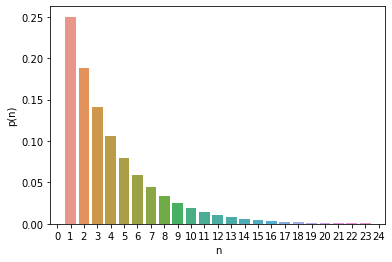
\includegraphics[width=\columnwidth]{solutions/ma/2017/46/figures/plot.png}
    \caption{PMF of $X$  }
    \label{ma2017-46:beta}
\end{figure}



%
\item Let (X,Y) be a random vector such that, for any $y>0$, the conditional probability density function of X given $Y=y$ is $$f_{X|Y=y}(x)=ye^{-yx} \:,x>0. $$ If the marginal probability density function of Y is $$g(y)=ye^{-y}\:,y>0$$ then $E(Y|x=1)=$
\\
\solution
Given,
the conditional probability density function of X given $Y=y$,
\begin{align}
f_{X|Y=y}(x)=ye^{-yx} \:,x>0 \label{st2020-43:a}
\end{align}
and, the marginal probability density function of Y,
\begin{align}
g(y)=ye^{-y}\:,y>0 \label{st2020-43:b}
\end{align}
let the joint probability density function of (X,Y) be $f_{X,Y}(x,y)$.
We know that,
\begin{align}
f_{X|Y=y}(x)=\frac{f_{X,Y}(x,y)}{g(y)}  \label{st2020-43:c}
\end{align}
using \eqref{st2020-43:a} and \eqref{st2020-43:b} in \eqref{st2020-43:c},
\begin{align}
f_{X,Y}(x,y) =y^{2}e^{-y(x+1)} \:,x,y>0 \label{st2020-43:d}
\end{align}
let the marginal probability density function of X be $f_{X}(x)$,
as we know ,
\begin{align}
f_{X}(x)= \int_{0}^{\infty}{f_{X,Y}(x,y)}\,dy \label{st2020-43:e}
\end{align}
using \eqref{st2020-43:d} in \eqref{st2020-43:e},
\begin{align}
f_{X}(x) &=\int_{0}^{\infty}{y^{2}e^{-y(x+1)}}\,dy\\
&=\frac{2}{(x+1)^{3}} \:,x>0\label{st2020-43:f}
\end{align}
The conditional probability density function of Y given $X=x$ is given by,
\begin{align}
f_{Y|X=x}(y) =\frac{f_{X,Y}(x,y)}{f_{X}(x)} \label{st2020-43:g}
\end{align}
using \eqref{st2020-43:d} and \eqref{st2020-43:f} in \eqref{st2020-43:g},
\begin{align}
 f_{Y|X=x}(y) =\frac{y^{2}e^{-y(x+1)}(x+1)^{3}}{2} \:,x,y>0
\end{align}
The conditional probability density function of Y given $X=1$ is given by,
\begin{align}
 f_{Y|X=1}(y) =4y^{2}e^{-2y}  \:,y>0 \label{st2020-43:h}
\end{align}
We need to find $E(Y|X=1)$ which is given by,
\begin{align}
 E(Y|X=1) &= \int_{0}^{\infty}{yf_{Y|X=1}(y)}\,dy \label{st2020-43:i}
\end{align}
using \eqref{st2020-43:h} in \eqref{st2020-43:i},
\begin{align}
E(Y|X=1) &= \int_{0}^{\infty}{4y^{3}e^{-2y}}\,dy\\
  &= \left[\frac{-e^{-2y}(8y^{3} + 12y^{2} + 12y + 6)}{4}\right]_0^{\infty}\\
        &=\frac{3}{2}
\end{align}


\end{enumerate}
\end{document}
